\documentclass{standalone}
\usepackage{fontspec}
\setsansfont{DejaVuSans.ttf}[Path=./,Kerning=Off,Ligatures={TeXOff,NoCommon}]
\usepackage{tikz}
\begin{document}
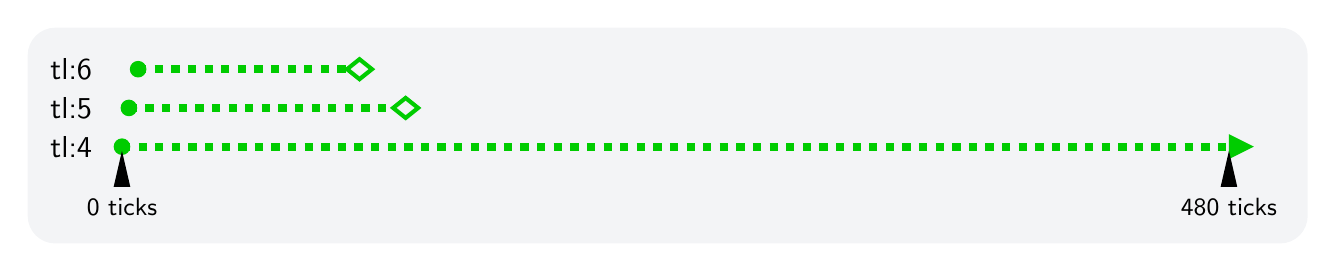
\begin{tikzpicture}[x=1pt,y=1pt,miter limit=4,font=\sffamily]
\definecolor{ts000000}{HTML}{000000}
\definecolor{ts00CC00}{HTML}{00CC00}
\definecolor{tsF3F4F6}{HTML}{F3F4F6}
\begin{scope}[shift={(16,16)}]
\path[rounded corners=10pt,fill=tsF3F4F6] (0,0) rectangle (462.5325,77.9766);
\path[draw=ts00CC00,line width=3pt,dash pattern=on 3pt off 3pt] (34.0737,34.9766) -- (434.0737,34.9766);
\path[fill=ts00CC00] (34.0737,34.9766) circle[radius=3];
\path[fill=ts00CC00] (443.0737,34.9766) -- (434.0737,39.4766) -- (434.0737,30.4766) -- cycle;
\path[draw=ts00CC00,line width=3pt,dash pattern=on 3pt off 3pt] (36.5737,48.9766) -- (132.0737,48.9766);
\path[fill=ts00CC00] (36.5737,48.9766) circle[radius=3];
\path[draw=ts00CC00,line width=1.5pt] (132.0737,48.9766) -- (136.5737,52.5766) -- (141.0737,48.9766) -- (136.5737,45.3766) -- cycle;
\path[draw=ts00CC00,line width=3pt,dash pattern=on 3pt off 3pt] (39.9071,62.9766) -- (115.4071,62.9766);
\path[fill=ts00CC00] (39.9071,62.9766) circle[radius=3];
\path[draw=ts00CC00,line width=1.5pt] (115.4071,62.9766) -- (119.9071,66.5766) -- (124.4071,62.9766) -- (119.9071,59.3766) -- cycle;
\path[fill=ts000000] (34.0737,33.4766) -- (31.0737,20.4766) -- (37.0737,20.4766) -- cycle;
\path[fill=ts000000] (434.0737,33.4766) -- (431.0737,20.4766) -- (437.0737,20.4766) -- cycle;
\node[anchor=base west,inner sep=0,font=\sffamily\fontsize{11}{12.8047}\selectfont,text=ts000000] at (8,59.1685) {tl:6};
\node[anchor=base west,inner sep=0,font=\sffamily\fontsize{11}{12.8047}\selectfont,text=ts000000] at (8,45.1685) {tl:5};
\node[anchor=base west,inner sep=0,font=\sffamily\fontsize{11}{12.8047}\selectfont,text=ts000000] at (8,31.1685) {tl:4};
\node[anchor=base,inner sep=0,font=\sffamily\fontsize{9}{10.4766}\selectfont,text=ts000000] at (34.0737,10.1226) {0 ticks};
\node[anchor=base,inner sep=0,font=\sffamily\fontsize{9}{10.4766}\selectfont,text=ts000000] at (434.0737,10.1226) {480 ticks};
\end{scope}
\end{tikzpicture}
\end{document}
